\subsection{Why the discrete and continuous constants differ}
\label{a:sec:compare}

The preceding bounds now settle the discrete--continuous comparison.  The two
constants are
\begin{equation*}
\Ac(p) = \frac{1-2p}{1-p}\quad\text{(continuous time)},
\qquad
A(p) = \lim_{n\to\infty}\frac{S_n}{(2p)^n}\quad\text{(discrete time)},
\end{equation*}
The continuous constant begins at $1$, whereas the discrete constant begins at
$\tfrac12$; nevertheless, halving the first does not superpose the two curves.

Equation \cref{a:prop:bounds} explains the discrepancy.  Rather than
$A=\tfrac12\Ac$, one has the strict inequality $A>\tfrac12\Ac$, with equality
approached only as $p\to0$.  Combining
\cref{a:eq:A-near-critical,a:eq:Acts}, the ratio runs monotonically across the
interval:
\begin{equation}
\label{a:eq:ratiolimits}
\frac{A(p)}{\Ac(p)} \;\longrightarrow\; \tfrac12 \quad(p\to0),
\qquad
\frac{A(p)}{\Ac(p)} \;\longrightarrow\; 1 \quad(p\to\tfrac12^-),
\end{equation}
taking the values $0.503$, $0.528$, $0.619$, $0.798$, $0.928$ and $0.988$ at
$p=0.01,\,0.1,\,0.3,\,0.45,\,0.49,\,0.499$.  Its variation rules out any constant
factor relating the two curves.

The two endpoint limits have distinct interpretations.  As $p\to0$, the factor of
two is a counting effect.  In the binary discrete model an
individual leaves either nothing or two offspring, so a surviving population is
always even (\cref{a:prop:parity}); deep in the subcritical regime, conditioning on
survival means conditioning on a population of exactly two, and the
quasi-stationary mean is $2$.  In the continuous-time model, by contrast, a
survivor is a single individual that has not yet died, giving a quasi-stationary
mean of $1$.  Their reciprocals are $\tfrac12$ and $1$, which accounts for the
discrepancy.

As $p\to\tfrac12^-$, the factor disappears because both constants obey the same
critical scaling.  Expanding \cref{a:eq:Acts} near $p=\tfrac12$ gives
$\Ac(p)=(1-2p)/(1-p)\to2(1-2p)$, precisely the leading term in
\cref{a:eq:A-near-critical}.  At this scale the discrete generational clock no
longer affects the leading order, and both models retain the same
$2\varepsilon$ behaviour.

The discrete curve is therefore squeezed between $\tfrac12\Ac$ and its critical
asymptote, approaching the former at one endpoint and the latter at the other.

\subsection{Searching for a closed form}
\label{a:sec:GA}

Before the connection in \cref{a:sec:koenigs} was recognised, several methods were
used to search for an elementary formula for $A(p)$.  Their failure is informative
because it separates visual agreement from the endpoint behaviour required by the
analysis above.

The first method used the continuum approximation developed in \ChM, treating the
map as a differential equation in the large-generation limit.  This recovers the
shape of the decay but leaves its constant of integration, and hence $A(p)$,
undetermined.

The second method was symbolic regression by genetic algorithm.  The procedure is
straightforward:
generate fifty candidate functions at random, measure how closely each reproduces
the target curve, retain the best five, and build a fresh population of fifty by
varying those; then measure again, and repeat the cycle of variation and selection
many times over \cite{stanley2002evolving,cohen2024physics}.  The first
implementation searched a space of polynomials, on the hunch that the answer might
take that form and because such functions are simple to encode: a genome is a
coefficient list $[a_0,\dots,a_k]$ for $a_0+a_1p+\cdots+a_kp^k$ up to some maximum
order, drawn uniformly at random.  The search quickly showed that many
substantially different formulae produce curves indistinguishable from the target
by eye. Supposing that a true formula might have rational coefficients, a second
version searched $\sum_i(a_i/b_i)p^i$ with $[a_i],[b_i]\in\mathbb Z^{k+1}$, and a
third extended the space to ratios of two such polynomials.  The strongest
candidates fitted the high-precision numerical data closely but did not satisfy the
analytic constraints.  For example,
\begin{equation}
\label{a:eq:A1hat}
\hat A_1(p) = \frac{\tfrac12(1-2p)(1+2p)}
{1+\tfrac12p-\tfrac52p^2-\tfrac65p^3+\tfrac65p^4} .
\end{equation}
This candidate passes through $(0,\tfrac12)$ and $(\tfrac12,0)$, yet fails the
diagnostic from \cref{a:eq:A-near-critical}: its derivative at $p=\tfrac12$ is
$-2/0.55=-3.636$, rather than the required $-4$.

A later attempt used a symbolic tree search over progressively nested elementary
functions.  It reached the same conclusion: functions of widely different form can
track the target closely, even when the search explicitly favours candidates with
fewer components.  The returned expressions typically nested trigonometric and
iterated exponential terms around a dozen or more fitted decimal constants, with no
useful interpretation.  One comparatively concise example is
\begin{equation}
\label{a:eq:A3hat}
\hat A_3(p) = \frac{-0.616647881739505\,\ee^{-0.552605335919693\,\ee^{p}}}
{\sin(\cos p)-|p|} + 0.921964323679771 .
\end{equation}

\begin{figure}[ht]
\centering
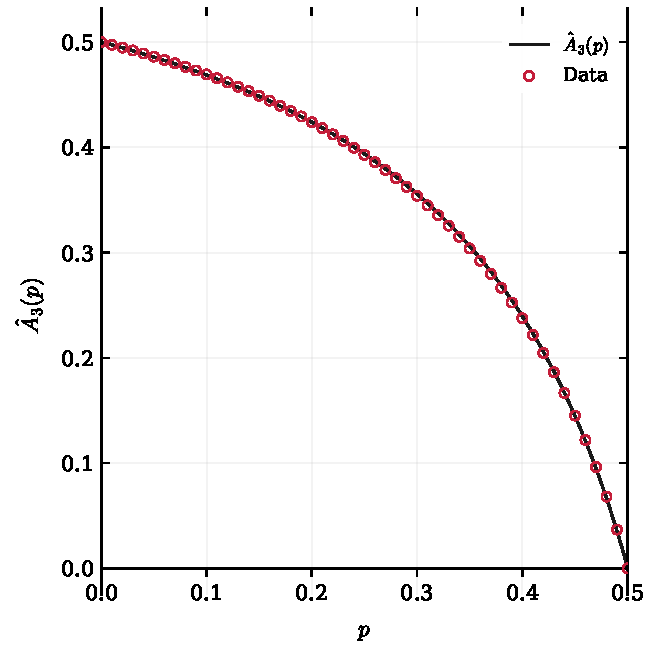
\includegraphics[width=0.56\textwidth]{figures/IMG_ch3/A3_hat_plot.pdf}
\caption{The symbolic-regression candidate $\hat A_3(p)$ of \cref{a:eq:A3hat}
(solid) against numerically computed values of $A(p)$ (red circles). The agreement
is excellent to the eye across the whole interval, which is exactly the problem:
the fit is not evidence of correctness. $\hat A_3$ misses the critical point,
returning $\hat A_3(\tfrac12) = 9.1\times10^{-4}$ rather than $0$, and arrives
there with gradient $-3.63$ instead of $-4$. Errors of this size are invisible here
but are fatal for $1/A$ near criticality.}
\label{a:fig:A3hat}
\end{figure}

The same defect recurs across these searches.  The candidates either fail to pass
through $(\tfrac12,0)$ or fail to arrive there with gradient $-4$, and near
criticality this distinction is decisive: as $A\to0$, an error in $A$ of vanishing
absolute size produces an $O(1)$, and eventually unbounded, error in the
quasi-stationary mean $1/A$.  A formula may therefore appear exact on a plot of
$A$ while remaining unusable for $1/A$.

A pragmatic patch is to splice the asymptotic onto a fitted curve,
\begin{equation}
\label{a:eq:A4hat}
\hat A_4(p) =
\begin{cases}
-0.04011483983619545\,\ee^{\ee^{2p}} + 0.6079994336528085, & p<0.499962,\\[2mm]
2-4p, & p\ge0.499962,
\end{cases}
\end{equation}
which repairs the critical regime.  Once a splice is admitted, however, the fitted
branch is better replaced by an exact representation; \cref{a:sec:practical}
develops that scheme.

These searches lead directly to the next section.  The abundance of distinct
formulae with nearly identical behaviour on a bounded interval is not evidence for
any particular closed form.  Curve fitting alone cannot distinguish a function
that has such a representation from one that does not.
